\documentclass{report}
\usepackage[T1]{fontenc}
\usepackage{lmodern}
\usepackage[utf8]{inputenc}

% Newline instead of indent for paragraph
\usepackage[parfill]{parskip}

% Bold \emph 
\renewcommand{\emph}[1]{\textbf{#1}}

% Description environment
\usepackage{enumitem}

% Math stuff like \DeclareMathOperator
\usepackage{amsmath}

% Algorithm desctiptions
\usepackage[ruled,vlined]{algorithm2e}

% Plots such as FAR/FRR
\usepackage{pgfplots}

% Links for TOC and refs
\usepackage{hyperref}

% References with name of item etc
\usepackage{cleveref}

\usepackage{todonotes}

\DeclareMathOperator{\hash}{hash}

\title{Lecture Notes: Security of IT-Systems}
\author{Jonas Otto}

\begin{document}

\maketitle

\listoftodos

\tableofcontents

\chapter{Fundamentals}
\section{Motivation and Introduction}
The number of catalogued vulnerabilities is rising rapidly over time, ever since
IT existed. Security is all over the headlines both in dedicated news agencies
and in mainstream media. Ransomware attacks are popular recently and have highly
visible and critical targets such as hospitals and large companies. Running a
networked computer system with 100\% security is neither feasible nor possible.
But strong security is still achievable, and defending most attackers is
possible.

\section{Terminology}
When talking about ``secure'' systems, what is usually desired is a
``dependability'', meaning a system that shows no unexpected or unacceptable
behavior. A dependable system should fulfill multiple goals, including
\begin{itemize}
    \item \emph{Availability}
    \item Reliability
    \item Safety
    \item \emph{Integrity}
    \item Maintainability
    \item \emph{(Confidentiality)}
\end{itemize}

The three major security goals are Confidentiality, Integrity and Availability
(\emph{CIA}). The main difference between dependability and security is that the
security is usually assessed from the viewpoint of a potential attack, while
dependability is considered in a more general context. Security can be seen as a
precondition of having a dependable system. A secure system is a system that can
achieve the three mentioned goals even facing an attacker.

\begin{description}[align=right,labelwidth=3cm]
    \item[Confidentiality] Protection of information against unauthorized access
    \item[Integrity] Protection against unauthorized change and destruction
    \item[Availability] Protection against rendering IT resources inaccessible
\end{description}

A \emph{threat} is defined by a potential error in the system, which could
enable an attacker to violate those objectives. A \emph{vulnerability} is a
concrete fault in the system that threaten one or more security objective. A
threat would be for example the possibility of a DDOS attack towards a web
service, a lack of resources to cope with the attack is a vulnerability. If an
attacker exploits the vulnerability, this is called an \emph{attack}.

The concepts of safety and security shall be differentiated.

When analyzing a system with regards to it security, two factors are considered:
The first is \emph{threat potential}, which estimates the likelihood of each
potential attack against the system. The second is the \emph{damage potential},
which asks what the impact to the system would be if an attack succeeds. Likely
high-impact attack scenarios can be mitigated by either reducing the impact of a
successful impact or by taking security measures reducing the likelihood of a
successful attack.

A few more useful definitions:
\begin{description}[align=right,labelwidth=3cm]
    \item[Identification] Assignment of an identifier
    \item[Authentication] Verification of an identity
    \item[Authorization] Assignment of permissions
    \item[Access Control] Protection of resources against unauthorized access
    \item[Privacy] Protecting personal information
\end{description}

\section{Attacks and Defenses}
\subsection{Attacks}
Attack can be categorized by many measures, like intention, approach or point of
attack.

Categories by intention can be:
\begin{description}
    \item[Denial of Service ]Making an IT system unabailable to users
    \item[Information Theft] Access to confidential information by unauthorized
          persons
    \item[Intrusion] Bypassing access control to gain access to a system
    \item[Tampering] Modification of stored or transmitted data
\end{description}

By approach:
\begin{itemize}
    \item Masquerading
    \item Eavesdropping
    \item Authorization Violation
    \item Loss/Modification
    \item Denial/Repudiation
    \item Forgery
    \item Sabotage
\end{itemize}

By point of attack:
\begin{itemize}
    \item Network
    \item Network services
    \item Operating system/Applications
    \item User
\end{itemize}

Another possible method of categorization is ``STRIDE'' categorization, which
stands for Spoofing, Tampering, Repudiation, Information disclosure, Denial of
Service and Elevation of privilege.

An attack often follows similar patterns. The first step is collecting
information of the system. This may expose a possible attack vector to the
attacker, which can then be used/tested. This is often repeated, as the first
attack is not necessarily successful. After a successful intrusion the next step
is often privilege escalation. This may allow the attacker to cover their
tracks, install back doors, etc. If the main goal of the attack is not reached
yet, this point may be used as the starting point for the next attack, towards
the initial goal.

Understanding and talking about attacks is vital when dealing with security, as
this is the very point we are trying to defend against.

\subsection{Security Mechanisms and Policies}
A Policy is a statement of what is, and what is not allowed. This allows the
distinction into ``authorized'' and ``unauthorized'' that we made already.

A Security mechanism is a method, tool or procedure that attempts to enforce
such policies. We can categorize those measures into prevention, detection and
recovery. It is possible to employ multiple measures, for example a gate as a
way of prevention, and a camera pointed at the gate which provides detection of
a successful attack.

\emph{Security through obscurity} or prohibiting reverse engineering and
attacking is not an alternative to real security.

Security mechanisms can never be judged by themselves. During risk assessment,
it is always necessary to evaluate the measures in the context in which they are
employed. The security of a system is determined by the weakest link in the
chain.

\chapter{Cryptography}
\section{Cryptographic Hash Functions and Random Numbers}
\subsection{Hash Functions}
A hash function is defined as a function $h: D \mapsto S$ with $|D| > |S|$. A
hash function is expected to fulfill more desired properties:
\begin{itemize}
    \item Compression: $|D| \gg |S|$
    \item Chaotic: Maximal change of the hash with minimal change in input
    \item Surjective: |S| is fully used
    \item Efficient calculation
\end{itemize}
Even with those properties, a hash function is not considered a cryptographic
hash function. Even a CRC fulfills those properties. The additional properties
of a \emph{cryptographic} hash functions are:

\paragraph{One way function:} Also called \emph{first pre-image resistance},
    this implies that given a hash, an input producing that hash can not be
    computed efficiently.

\paragraph{Weak collision resistance:} Also called \emph{second pre-image
    resistance}, implies that given a hash $h = \hash(m)$, an input $m' \neq m$
    with $\hash(m') = h$ can not be efficiently found.

\paragraph{(Strong) collision resistance:} No $m$ and $m' \neq m$ can be found
    efficiently with $\hash(m) \neq \hash(m')$. In contrast to weak collision
    resistance, a specific hash value is not required here.

Hash functions can be used in combination with a key in the form of
\emph{Message Integrity Code} and \emph{Message Authentication Code} to provide
an equivalent to digital signatures using symmetric cryptography. The hash based
MAC \emph{HMAC} is calculated as a hash over a combination of the message with a
key.

\subsection{Random Number Generators}
Pseudo-Random Number Generators \emph{PRNG}s which produce a deterministic
sequence of numbers from an initial seed are not suitable for cryptographic
applications such as key generation due to their predictability.
Non-Deterministic RNGs exist and often rely on external physical processes like
noise in electronic circuits. They do however often have a low data rate which
is not sufficient for all applications. A combination of a PRNG which is
(periodically) seeded by a true, non-deterministic RNG is an approach used in
practice.

Criteria for good RNGs are:
\begin{itemize}
    \item Statistical distribution as desired
    \item Independence: No repeating sequences, invariant to environmental
          conditions
    \item Speed of generation
    \item Long periodicity (PRNGs) / Non-reproducibility
\end{itemize}


\section{Encryption}
One important distinction between encryption schemes is the concept of symmetric
and asymmetric ciphers. Symmetric encryption is also called secret key
cryptography and relies on the presence of a secret key at both endpoints of the
communication. Asymmetric or public key encryption separates the key into a
public and private key for both parties. Information about the secret key is
never shared, and it can be used to decrypt messages which are encrypted using
the corresponding public key.

The algorithm itself is never considered secret, the security shall only depend
on the secret keys (Kerckhoffs principle).

Additional actors in a encryption scheme that are to be considered are the
passive (eavesdropping) attacker (\textit{Eve}), the active (man-in-the-middle)
attacker (\textit{Mallory}) and a trusted third party (\textit{Trent}).

\subsection{Symmetric Encryption}
Symmetrical encryption approaches usually follow the pattern of using basic
bitwise operations to form building blocks such as Feistel networks which are
then combined or repeated in multiple rounds. A challenge arises when the input
of the cipher is of variable length. Stream ciphers are suited to such a
problem, but the more common approach is to divide the input into blocks and use
a block cipher, operating with a fixed input size, multiple time. Simply
applying the same cipher with the same key to each block (\textit{electronic
code book}) however is not a good approach since repeated blocks in the input
will be directly reflected in the ciphertext. Alternatives include integrating
the previous ciphertext into the next block or including a counter in each
block, to avoid repeating inputs to the cipher altogether.

A standard block cipher used today is the \textit{Advanced Encryption Standard}
\emph{AES}, a block cipher with variants for different key lengths such as 128,
192 or 256 bit.

\subsection{Asymmetric Encryption}

Asymmetric encryption makes encryption possible even without a previously agreed
on private key.

\subsection{Diffie-Hellman Key Exchange}
The goal of the DIffie-Hellman key exchange algorithm is to establish a private
key between two users Alice and Bob, without compromising the secret key to an
attacker that has full visibility of the entire communication between Alice and
Bob.

\begin{algorithm}
    \SetAlgoLined
    
    \KwResult{private key $k$}
    choose public modulus $p$ (prime)\;
    choose public base $g$ (primitive root modulo $p$)\;
    \Begin(Alice){
        choose secret $a$\;
        $A = g^a \mod p$\;
        publish $A$;
    }
    \Begin(Bob){
        choose secret $b$\;
        $A = g^b \mod p$\;
        publish $B$\;
        $k = A^b \mod p$\;
    }
    \Begin(Alice){
        $k = B^a  \mod p$\;
    }
    \caption{Diffie-Hellman Key Exchange}
\end{algorithm}

This results in the same private key $k$ for both Alice and Bob. Generating this
private key requires knowledge of one of the secrets $a$ or $b$, which are only
known to the corresponding party.

Diffie-Hellman itself is not secure against \emph{Man-in-the-Middle Attacks}. If
an attacker \textit{Mallory} intercepts the communication, they could perform a
separate key exchange with both Alice and Bob. They would both have a shared key
with Mallory, unaware that the real communication partner is not Alice or Bob.
Mallory can then decrypt incoming messages, read or modify them, and re-encrypt
them using the second key.

\subsection{RSA}
RSA is an encryption scheme which allows encrypted communication without first
establishing a symmetric secret key (using Diffie-Hellman for example). Each
participant calculates both a public key and a secret key. The public key can be
used by any participant to encrypt messages, which can only be decoded using the
corresponding secret key, which is only known to the owner of the key.

\subsection{Digital Signatures}
If the integrity of a document and identity of the author are of concern, but
the contents are not necessarily encrypted, digital signatures are used. In
digital signatures, the signature is generated for a specific message (usually a
hash of the document) with the private key of the author. The verification of
the signature is possible using the corresponding public key and again the
message. This is similar to the reverse of the public key encryption scheme.

\subsection{Strength of Cryptographic Approaches}
The security of cryptographic algorithms can be categorized in the following
categories:

\begin{itemize}
    \item \textbf{Empirically secure:} The approach is secure because no attacks
    against it have been successful, and analysis has not found a specific
    weakness
    \item \textbf{(Formally) proven secure:} The encryption is proven to be a
    mathematically hard problem
    \item \textbf{Unconditionally secure:} ``An attacker cannot extract any
    information from the encrypted text''
\end{itemize}

The only unconditionally secure approach is the \emph{one-time pad}, where the
key and message have the same length and a unique, random key is used for every
transmission. Since the key has no inherent correlation, the probability of
recovering any arbitrary plaintext is identical, which makes even brute force
attacks impossible.

\chapter{Identification and Authentication}
\label{chapter:authentication}
\section{Identification}
The identity of an entity shall have the following properties:
\begin{itemize}
    \item Uniqueness
    \item Unchangable Linking
    \item Lifelong validity
    \item No Transferability
\end{itemize}

In order to identify an entity, an \emph{identifier} has to be defined. The
identifier should meet the above criteria and should be able to determine an
identity \textit{within a given context}.

Identifiers have the purpose of both accountability and access control. They
can be applied to both subjects (users, processes, ...) and objects (files,
URLs, ...), humans and machines, and can be temporary or persistent.

For authentication, a separate \textit{proof of identity} is usually required:

\section{Authentication}
Authentication is the process of confirming whether a second party is indeed who
they claim to be, to a specified level of confidence. There are three basic
forms of authentication:

\begin{itemize}
    \item \emph{Something you know} (passwords)
    \item \emph{Something you have} (smart cards)
    \item \emph{Something you are} (biometrics)
\end{itemize}

Combinations of those increase the security
(\emph{Multi-Factor-Authentication}).

\paragraph{Password Authentication} is based on the \textit{something you know}
factor. Examples include unix passwords, PINs or secret code words. They can
also easily be used to authenticate groups, by distributing the password to
every entity in the group. A weakness of passwords is that an attacker can learn
and reuse it. A possible solution are \textit{one-time passwords}.

\paragraph{One-time Passwords} are only used once, an example would be a TAN
list for online banking. They can also be part of a challenge-response-protocol,
where the two parties agree on a secret function beforehand, and authentication
happens by verifying the function response to a challenge.

\paragraph{Hardware Tokens} take a similar approach in generating some kind of
one-time use token, but those are generated by dedicated hardware, shifting the
factor to \textit{something you have}. They might have an additional input such
as a pin, or, as in the case of popular 2FA solutions, the current time. The
\emph{HOTP} (HMAC-based One-Time Password algorithm) generates short time
passwords using a counter (time) and a pre-shared secret key.

\paragraph{Biometric Authentication} has to be differentiated into
\textit{verification} and \textit{recognition}. In verification, the used
specifies its identity, and the system authenticates the used if biometric
verification succeeds. In recognition, the system recognizes the user amongst
multiple known users without further input.

Biometric authentication systems can fail in two ways: \emph{False negative}
means that a user is incorrectly rejected, a \emph{false positive} means that a
user is wrongly accepted. The threshold on accepting a authentication attempt
has to be chosen in a application specific way, depending on which fault is more
acceptable. \Cref{fig:eer} shows the relationship between the
\textit{False Acceptance Rate} and \textit{False Rejection Rate} with a varying
threshold. A measure of the security of the authentication system could be the
\textit{Equal Error Rate}.
\begin{figure}
    \centering
    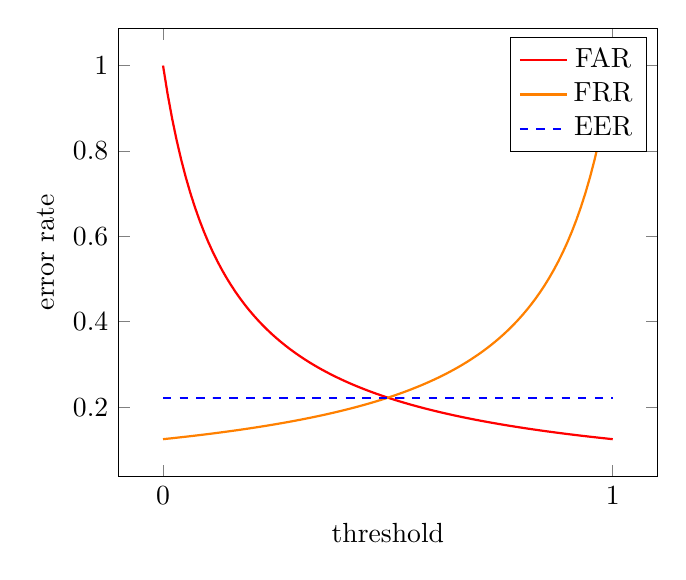
\begin{tikzpicture}
        \begin{axis}[
                xlabel=threshold,
                ylabel=error rate,
                xtick={1,8},
                xticklabels={0,1}
            ]
            \addplot[
                domain=1:8,
                samples=100,
                thick,
                color=red]{1/x};
            \addlegendentry{FAR};
    
            \addplot[
                domain=1:8,
                samples=100,
                thick,
                color=orange]{1/(9-x)};
            \addlegendentry{FRR};
    
            \addplot[
                domain=1:8,
                samples=100,
                dashed,
                thick,
                color=blue]{2/9};
            \addlegendentry{EER};
        \end{axis}
    \end{tikzpicture}
    \caption{\textit{False Acceptance Rate} and \textit{False Rejection Rate}
    for biometric authentication}
    \label{fig:eer}
\end{figure}

\section{Password Security}
Passwords which are short or badly chosen can easily be cracked. Brute-force or
dictionary attacks guess the password either randomly of from a list of known
(pass-)words. Brute-force attacks are easily feasible for passwords up to
\textasciitilde 8 characters in length, useful rules on possible guesses and
dictionary attacks can lead to success for even longer passwords. An advantage
for the attacker is when the attack can be executed \textit{offline}, such as by
stealing the file containing the password hashes. This removes the bottleneck of
the authentication mechanism of the target and allows for distributed attacks.

A common protection measure is to use a \emph{SALT}. A salt is a random value
that gets appended to the password before hashing, and then gets stored
alongside the password hash. While this does not protect a single password
against the mentioned attacks, it prevents reuse of a hash that has already been
calculated. Otherwise, it would be possible to just compare the hashes to known
hashes of popular passwords.

Another consideration is access to the password hashes. While the actual
cryptographic security is only influenced by the hash function, preventing
offline attacks by properly protecting the hashes forces the attacker to execute
much slower online attacks. Those online attacks can be slowed even further by
limiting the number of invalid authentication attempts or introducing an
increasing delay after failed authentication attempts (\textit{back off}), and
by using ``slow'' hash functions. The previously popular measure of password
aging (requiring passwords to be changed after a certain amount of time) is
discouraged, since it promotes the use of weak but easy to remember passwords.

Other attacks focus on the specific implementation of the authentication
mechanism and exploit vulnerabilities that allow login even without actually
obtaining the correct password, or allow changing or resetting passwords even
with insufficient privileges.

\subsection{Time Memory Trade-off}
In attacks on passwords a trade-off between time and memory has to be made, the
two extremes being the brute-force attack and the fully pre-calculated
dictionary/codebook attack.

One possible solution is a \emph{Variable Length Lookup Table}. Those rely on
hash chains: For many initial values, a chain of hashes (length $n_\text{max}$)
each is calculated. Only the initial and end-value are for each chain is then
stored. When a certain hash shall then be cracked, it will be hashed
$n_\text{max}$ times until a chain is found which end-state matches the
calculated hash. Once the chain is found, it can be restored using the stored
initial state which results in a chain containing the to-be-cracked hash and the
password as the state immediately preceding that value.

An improvement to lookup time can be made by making the chains variable length,
and introducing an end criterion, for example a certain number of zero-bits at
the end of the hash (\emph{Distinguished Codepoints}). This reduces the number
of end-lookups significantly.

Duplication arising from hash collisions are addressed by \emph{Rainbow Tables}:
A round-specific reduction function (hash space \textrightarrow password space)
is introduced. So even if a state is already present in a different chain (but
at another round in the chain), the original chain continues separately.

\section{Network Authentication}
\todo[inline]{Authentication: Network Authentication}

\todo[inline]{Chapter 4: Access Control}
\todo[inline]{Chapter 5: Malware}
\todo[inline]{Chapter 6: OS Security}
\todo[inline]{Chapter 7: Embedded, HW Security}
\todo[inline]{Chapter 8: Software Security}
\todo[inline]{Chapter 9: Network Security}
\todo[inline]{Chapter 10: Web security}
\todo[inline]{Chapter 11: Privacy}

\end{document}